\documentclass{article}
\usepackage[a4paper, total={6.77in, 10.69in}]{geometry}
\usepackage{graphicx}
\graphicspath{{../images/}}

\title{Database Schema}
\author{Adrian Prawira Susanto and Kevin Pratama and Randitya Setyawan Mohamad}
\date{}
\begin{document}
    \maketitle \medskip
    \begin{center}
        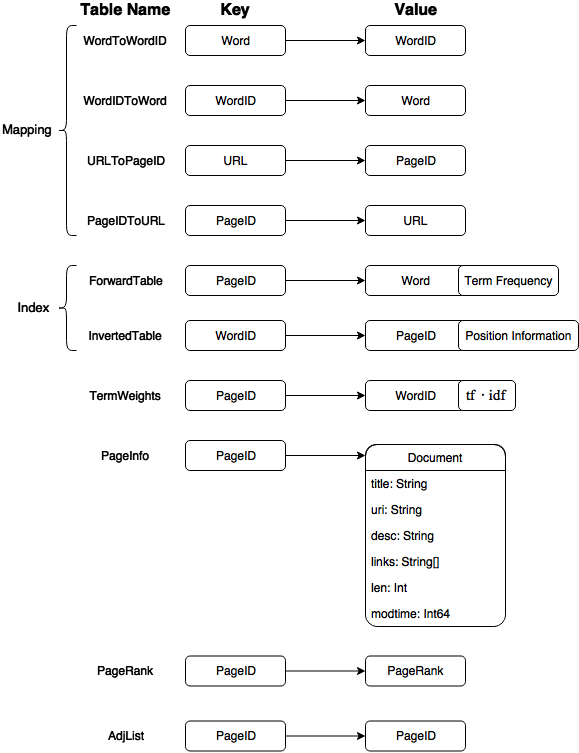
\includegraphics[scale=0.5]{databaseSchema} \\[2\baselineskip]
    \end{center}
    The package used for our database manager is Bolt for Go, which is a pure key/value storage package for Google's Go Language.
    As for the schema itself, we partititioned the tables into three big groups:
    \begin{enumerate}
        \item Mappings \\
        These tables contain convenient mapping from one value to another, to allow ease of use during implementation.
        \item Indexes \\
        These tables are one of the most integral part of our search engine. The indexes allow for both forward lookup (From DocumentID to the words) and backward lookup (From Word to DocumentID), commonly known as Forward and Inverted index respectively.
        \item Miscellaneous \\
        These tables contain extra information which are used ubiquituously in the program. TermWeights, for example, store each term weights ($tf \cdot idf$), which were precomputed to allow faster retrieval during runtime. PageInfo stores each document information which then are processed to the indexes, or used during crawling. AdjList, as can be referred from its name, stores the adjacency list of the indexed pages. From this AdjList, PageRank of each pages can be obtained and precomputed, which are then stored in the table PageRank.
    \end{enumerate}

\end{document}